\textcolor{red}{\textbf{Conceitos trabalhados}: informação de Fisher; estimador de máxima verossimilhança; reparametrização; admissibilidade; eficiência.}\\ \textcolor{purple}{\textbf{Nível de dificuldade}: médio.}\\
\textcolor{blue}{
\textbf{Resolução:}
Para facilitar, vamos estabelecer alguns fatos antes de começar a resolução.
Primeiro, se $W$ é uma variável aleatória com distribuição Poisson com taxa $\lambda$, então
\begin{align*}
    E_\theta[W^2] &= \vr_\theta(W) + (E_\theta[W])^2,\\
    &= \theta + \theta^2,\\
    & = \theta(1+ \theta).
\end{align*}
Além disso, se $\bX = (\rs)$ é um vetor de observações com média amostral $\bar{X}_n =  \frac{1}{n}\sum_{i=1}^n X_i$, então
\begin{align*}
    S_2 &:= \sum_{i=1}^n \left(X_i -\bar{X}_n\right)^2,\\
    & = \sum_{i=1}^n X_i^2 - 2 \bar{X}_n \sum_{i=1}^n X_i  + n\left(\bar{X}_n\right)^2,\\
    &= \sum_{i=1}^n X_i^2  -n\left(\bar{X}_n\right)^2,
\end{align*}
onde a penúltima linha segue do fato de que $S_n = \sum_{i=1}^n X_i = n \bar{X}_n$.
Armados destes fatos, vamos responder a).
Primeiro,
\begin{align*}
    E_\theta[\delta_1(\bX)] &= \frac{1}{n}\sum_{i=1}^n X_i,\\
    &= \frac{n\theta}{n} = \theta,
\end{align*}
portanto $\delta_1$, que é o estimador de máxima verossimilhança de $\theta$, é não-viesado.
Agora,
\begin{align*}
    E_\theta[\delta_2(\bX)] &= \frac{1}{n-1}\left\{\sum_{i=1}^n X_i^2 -n\left(\bar{X}_n\right)^2\right\},\\
    &= \frac{1}{n-1}\left\{n\theta(1+\theta) -nE_\theta\left[\left(\bar{X}_n\right)^2\right]\right\},\\
    & = \frac{1}{n-1}\left\{n\theta(1+\theta) -\frac{n}{n^2}E_\theta\left[\left(\sum_{i=1}^n X_i \right)^2\right]\right\},\\
    &= \frac{1}{n-1}\left\{n\theta(1+\theta) -\frac{n}{n^2}n\theta(1 + n\theta)\right\},\\
    &= \frac{\theta}{n-1}\left\{n(1+\theta) -(1 + n\theta)\right\},\\
    &= \theta.
\end{align*}
Para b) e d), precisamos calcular $I_n(\theta) = nI(\theta)$, e podemos fazer assim porque nossa amostra é i.i.d.
Assim,
\begin{align*}
    I(\theta) &= E_\theta\left[-\frac{\partial^2\theta}{\partial\theta^2}\log f_n(\bx \mid \theta)\right],\\
    &= E_\theta\left[-\frac{-\sum_{i=1}^n X_i}{\theta^2}\right],\\
    &= \frac{1}{\theta},
\end{align*}
de modo que $I_n(\theta) = n/\theta$ e portanto o limite inferior de Cramér-Rao para a variância de estimadores não-viesados de $\theta$ é $1/I_n(\theta) = \theta/n$.
Precisamos verificar se a variância de $\delta_1$ ``encaixa'' nessa cota.
\begin{align*}
    \vr_\theta(\delta_1(\bX)) &= \vr_\theta(\bar{X}_n),\\
    &= \frac{\vr_\theta(\sum_{i=1}^nX_i)}{n^2},\\
    &= \frac{n\theta}{n^2},
\end{align*}
o que mostra que a cota inferior é alcançada e, portanto, $\delta_1$ é eficiente.
Note também que $\lim_{n\to\infty}\bar{X}_n = \theta$, portanto $\delta_1$ também é consistente.
Outra maneira de ver isso é perceber que o viés de $\delta_1$ é zero e sua variância converge para zero assintoticamente\footnote{Lembre-se: convergência em média quadrática implica convergência em probabilidade, como vimos na revisão de Probabilidade no início do curso.}.
Agora, vamos resolver c), o que implica computar a variância de $\delta_2$, $\vr_\theta(\delta_2(\bX)) = E_\theta\left[\{\delta_2(\bX)\}^2\right] -\theta^2$.
Vamos reescrever $\delta_2$ para nos facilitar a vida:
\begin{align*}
    \delta_2(\bX) &= \left(X_1 - \frac{X_1 + X_2}{2}\right)^2 + \left(X_2 - \frac{X_1 + X_2}{2}\right)^2,\\
    &= \left(\frac{X_1 - X_2}{2}\right)^2 + \left(\frac{X_2 - X_1}{2}\right)^2,\\
    &= 2\frac{(X_1-X_2)^2}{4} = \frac{(X_1-X_2)^2}{2}.
\end{align*}
Estamos em posição de calcular
\begin{align*}
\vr_\theta(\delta_2(\bX)) &=  E_\theta\left[\{\delta_2(\bX)\}^2\right] -\theta^2,\\
 &=  E_\theta\left[\left\{\frac{(X_1-X_2)^2}{2}\right\}^2\right] -\theta^2,\\
&= 3\theta^2 + \frac{\theta}{2}-\theta^2,\\
&= 2\theta^2 + \frac{\theta}{2},
\end{align*}
onde a penúltima igualdade segue da dica dada.
Como $2\theta^2$ é positivo necessariamente, concluímos que $\delta_2$ não é eficiente; como demonstramos que existe outro estimador não-viesado que é de fato eficiente, somos forçados a concluir que $R(\delta_2, \theta) > R(\delta_1, \theta)$ para todo $\theta$ e, que portanto, $\delta_2$ não é admissível.
A Figura~\ref{fig:poisson_ests} mostra um esboço da distribuição de $\delta_1$ e $\delta_2$ para $n=2$ e $\theta_0 = \zeta(3) \approx 1.2021$.
\begin{figure}[!ht]
\begin{center}
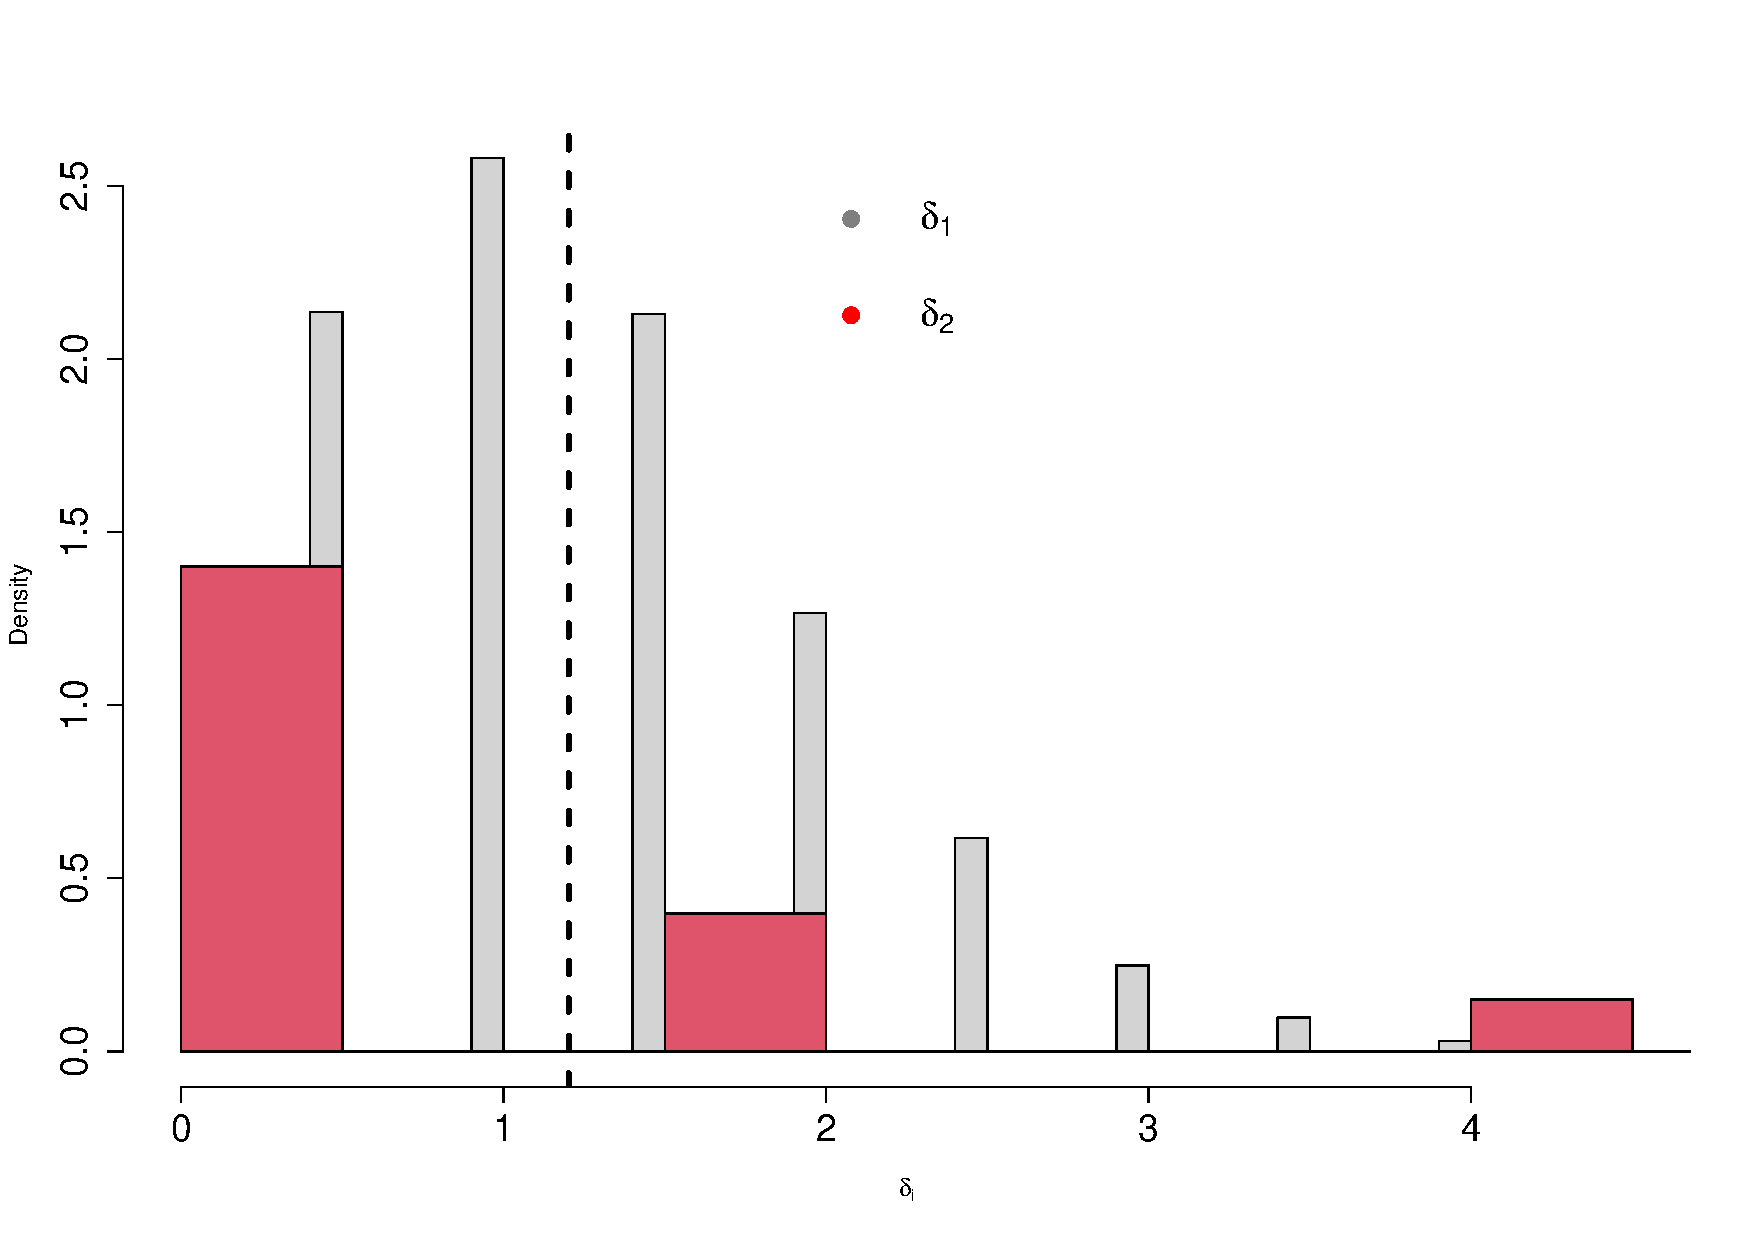
\includegraphics[scale=0.4]{Q2_A1_2022_ests.pdf}    
\end{center}
\caption{\textbf{Distribuição amostral dos estimadores $\delta_1$ e $\delta_2$ no caso Poisson}.
Mostramos os histogramas para $N=5000$ simulações de Monte Carlo com $\theta_0 = 1.2021$ -- marcado pela linha tracejada vertical.
Para estas simulações, $\vr(\delta_1) \approx 0.60$, enquanto $\vr(\delta_2)  \approx 3.49$.
}
\label{fig:poisson_ests}
\end{figure}
Para finalizar e responder e), vamos usar a dica para calcular $g^\prime(\theta) = 1/2\sqrt{\theta}$, o que nos leva a
\begin{align*}
    \frac{1}{\theta} = \frac{I_X(\eta)}{4\theta}
    \implies I_X(\eta) = 4, \: \forall \theta \in (0, \infty),
\end{align*}
o que de fato é constante com relação ao parâmetro, $\theta$.
Para ter certeza, vamos reparametrizar a p.m.f.  e proceder aos cálculos.
Note que $\theta = \eta^2$, portanto,
\begin{equation*}
    f_\eta(x) = \frac{\eta^{2x}e^{\eta^2}}{x!},
\end{equation*}
de modo que
\begin{equation*}
   \log f_\eta(x) = 2x \log(\eta) -\eta^2,
\end{equation*}
e 
\begin{equation*}
   \frac{\partial^2}{\partial\eta^2}\log f_\eta(x) = -\frac{2x}{\eta^2}-2.
\end{equation*}
Tomando menos a esperança da expressão acima, temos
\begin{equation*}
    I_X(\eta) = \frac{2E_\eta[x]}{\eta^2} + 2 = \frac{2\eta^2}{\eta^2} + 2 = 4.
\end{equation*}
$\blacksquare$\\
\textbf{Comentário:}
 Extraído do exercício 3, Seção 8.8, do DeGroot, e dos exemplos 8.7.5 e 8.8.8. A Seção 3.7 do livro The Bayesian Choice contém os detalhes do item (e). 
 O interessante aqui é que como na Poisson a média e a variância coincidem em termos do valor do parâmetro, então podemos criar dois estimadores de momentos, baseados na média e variância amostrais, respectivamente, para tentar estimar $\theta$.
 No entanto, apenas um deles será eficiente, o que nesse caso coincide com o estimador de máxima verossimilhança.
 Vimos também que a parametrização influencia fortemente a forma da informação de Fisher, e este é um fato que pode ser explorado. 
 Mais à frente no curso veremos as chamadas transformações estabilizadoras da variância e o método Delta, que ilustram esse ponto.
}